\documentclass[11pt]{article}
\usepackage{url}
\usepackage{graphicx,DCCN2018_en}

\pagestyle{fancy} % All pages have headers and footers
\fancyhead{} % Blank out the default header
\fancyfoot{} % Blank out the default footer

\usepackage[utf8]{inputenc}
\linespread{1.0}

\usepackage{amsmath}

\makeatletter
\fancyhead[RO]{\small DCCN 2018\\ {17-21 September 2018}}
\fancyhead[LO]{\small E. Yu. Shchetinin, et al.\\Short version of the article title}

\c@page=1 % Number will be set by publisher.
       
\makeatother


% Full title of the paper in English
\title{Development of an effective algorithm for short-term forecasting of 
  power consumption using ensemble}
%Author's (co-authors') name(s)
\author[1]{\small E. Yu. Shchetinin}
\author[2]{\small M. V. Berezhkov}
\author[2]{\small P. G. Lyubin}
%Affiliations:
\affil[1]{\footnotesize All-Russian Research Institute\\
  for Civil Defense and Emergencies of the MESRF\\
  (Science and High Technology Federal Center)\\
  Davydkovskaya str., 7, Moscow, 121352, Russia}
\affil[2]{Moscow State University of Technology ``STANKIN'',\\ 
  Vadkovsky lane, 3a, Moscow, 127055, Russia}

\email{\url{lyubin.p@gmail.com}, \url{riviera-molto@mail.ru}}
%%%%%%%%%%%%%%%%%%%%%%%%%%%%%%%%

\begin{document}

%Specify the UDC index corresponding to the topic of your work.
\udc{123.456}

{\let\newpage\relax\maketitle}
%\maketitle
\vskip -1.5em
\footnotetext{The publication has been prepared with the support of ... according to the research project No.{12345.67890}.}


%%%%%%%%%%%%%%%%%%%%%%%%%%%%%%%%%%%%%%%%%%%%%%%%%%%%%%%%%%%%%%
\begin{abstract}
Short-term forecasting of electricity consumption is an actual task in many
areas of human activity due to the specificity: consumers and power companies
can't accumulate energy and can't store energy. At the first, consumers which
participating in the wholesale electricity market must to submit a plan of
future consumption, and energy-generating companies need to plan the output.
Secondly, this indicator can be used as one of the features when fitting other
models. At the same time, the consumption of electrical energy by any object is
a time series, since it represents the instantaneous values of the consumed
power measured at different times with a certain periodicity. In article we
demonstrate a simple and effective method for short-term forecasting of power
consumption. The approach is based on the method of base models ensemble (RPART
- Recursive PARTitioning, CTREE - Conditional Inference Trees
\cite{BreimanEtAl}) and has a good prediction level comparable with more complex
algorithms. The ensemble method is an algorithm for combining a set of trained
models to improve the accuracy of the forecast with trying to avoid overfitting.
There are several ensemble methods that have their disadvantages and advantages.
We used Bagging (Bootstrap aggregating \cite{Breiman1996}) which helped to
improve the predictive power of particular base models.

\keywords{short-term forecast, ensemble, RPART, CTREE, random trees, power
consumption, bagging}
\end{abstract}
%%%%%%%%%%%%%%%%%%%%%%%%%%%%%%%%%%%%%%%%%%%%%%%%%%%%%%%%%%%%%%


\section{Introduction}
The most common methods of time series forecasting are:
\begin{itemize}
    \item extrapolation
    \item expert (intuitive) methods
    \item correlation and regression analises
    \item ARIMA-based methods
    \item adaptive methods
    \item Neural Network
    \item Hibryd Network
\end{itemize}

These methods can be used to predict electricity consumption and have inherent advantages and disadvantages. In modern works, more often than others, solutions of this problem are described with the use of artificial neural networks.


\subsection{Subsection heading here}

Subsection text here. Maximum level of depth allowed for defining sections is 2.


\section{General guidelines on the submitted paper}

The full text paper (3--8 pages) in PDF using current \LaTeX{} template have to be submitted to the DCCN organizing committee.

The name of the PDF-file should be combined of the surnames of the co-authors:
\textbf{Surname1\_Surname2\_Surname3.pdf}.

\section{Font}

Type the text of the paper in 11 points (11pt), regular. Each
paragraph is to be indented 5~mm, and their intervals must be 0
points before and after.

\section{Mathematical formulae and references}

To make references to mathematical expressions, it is
recommended to use \LaTeX{} mechanism. For example, the formula
given below
\begin{equation}
\label{eq:1}
P(n,t)=\frac{\partial^n B(t)}{\partial t^n}
\end{equation}
can be referred as \eqref{eq:1}.

\section{Theorems and proofs}

Theorems are defined like follows
\begin{thm}\label{thm1}
Text of the theorem.
\end{thm}

\begin{proof}
Proof of Theorem \ref{thm1}. If using such reference, you need
to recompile your paper with \LaTeX{} twice.
\end{proof}

\begin{coroll}
Corollary to theorem~\ref{thm1}
\end{coroll}

Lemmas are defined like follows
\begin{lem}\label{lem1}
Text of the lemma.
\end{lem}

Examples are defined like follows
\begin{example}
Text of the example.
\end{example}

\begin{remark*}
All \LaTeX{} theorem-like environments can be defined as unnumbered, by using the \verb"*"  symbol. For instance, \verb"\begin{remark*}...\end{remark*}".
\end{remark*}

\section{Figures and tables}

Figures should be provided in PDF or EPS format. Raster pictures have
to be made with maximal resolution (minimal 600 dots per inch).

\begin{figure}[ht!]
   \centering
     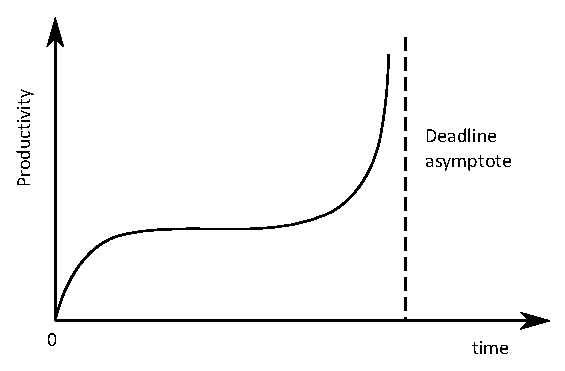
\includegraphics[width=0.8\textwidth]{funny_graph_en}
    \caption {Figure example}
\label{fig:example_graph}
\end{figure}

Below is an example of a table (see table~\ref{tab:sampletable}) with the title, formatted with the use of \verb"\caption".

\begin{table}[ht!]\begin{center}
\begin{tabular}{|c||c|c|c||c||c|c|c|}\hline
  Parameter & T & E & $\Delta$, \% & Parameter & T & E & $\Delta$, \% \\ \hline \hline
  $\rho_{1}^{(1)}$ & 0,187 & 0,194 & 3,7 &  $\rho_{1}^{(2)}$ & 0,127 & 0,120 & 5,6 \\ \hline
  $\rho_{2}^{(1)}$ & 0,073 & 0,072 & 1,4 &  $\rho_{2}^{(2)}$ & 0,052 & 0,053 & 1,9 \\ \hline
  $\rho_{3}^{(1)}$ & 0,148 & 0,147 & 0,7 &  $\rho_{3}^{(2)}$ & 0,103 & 0,103 & 0,0 \\ \hline
  $\rho_{4}^{(1)}$ & 0,036 & 0,036 & 0,0 &  $\rho_{4}^{(2)}$ & 0,026 & 0,027 & 3,7 \\ \hline \hline
  $C^{(1)}$ & 0,479 & 0,476 & 0,6 & $C^{(2)}$ & 0,656 & 0,640 & 2,5 \\ \hline \hline
  $C_{1}^{*}$ & 0,341 & 0,339 & 0,6 & $C_{3}^{*}$ & 0,323 & 0,329 & 1,8 \\ \hline
  $C_{2}^{*}$ & 0,296 & 0,298 & 0,7 & $C_{4}^{*}$ & 0,286 & 0,286 & 0,0 \\ \hline
\end{tabular}\caption{Table example}\label{tab:sampletable}
\end{center}\end{table}

The figures and tables must be numbered, have a self-contained
caption and referred in the main text. Figure and table
captions are placed below the object and centered. Also, avoid
placing figures and tables before their first mention in the
text. Use the abbreviation "Fig." even at the beginning of a
sentence.

The authors are recommended not to use characters smaller than
9 points (9pt) in figures. Do not use abbreviations in the titles
unless they are unavoidable.

\section{List of references}
The full list of references should be placed at the end of the paper in a
separate section. Citations inserted in the text should use square
brackets and the ordinal number of the item. To cite a paper one should use the \verb"\cite" command.  List
the references according to the order of their appearance in
the text.

The bibliography can be placed either using \verb"bibtex", or the \verb"thebibliography" environment. 


\section{Conclusion}
The Conlusions section should contain a brief summary of the content and purpose of the paper, reflecting its novelty and practical significance, proposals for practical implementation of research results and providing the final word on the value of your paper.

%You may use bibtex.
%\bibliographystyle{elsarticle-num}
%\bibliography{biblist}

\begin{thebibliography}{99}
\bibitem{bib1}  %% citation code
Bianchi G. Performance Analysis of the IEEE 802.11 Distributed
Coordination Function ~// IEEE Journal on Selected Areas in
Communications. 2000. V. 18. P.~535--547.

\bibitem{bib2} Vishnevsky V.~M., Lyakhov A.~I. IEEE 802.11
    Wireless LAN: Saturation Throughput Analysis with Seizing
    Effect Consideration
// Cluster Computing. 2002. V. 5. P. 133--144.

\bibitem{bib3} Neuts M.~F.  Structured Stochastic
    Matrices of M/G/1 Type and Their Applications. Marcel
    Dekker, New York, 1989.

\bibitem{bib4} Schriber T.~J. Simulation using GPSS. John
    Wiley \& Sons, 1974.
    
\bibitem{bib5} National Center for Biotechnology Information, \url{http://www.ncbi.nlm.nih.gov}

\end{thebibliography}

\end{document}
